\RequirePackage[l2tabu, orthodox]{nag}

\documentclass[
    a4paper,
    12pt,
    twoside,
    open=right,
    DIV=13,
    BCOR=15mm,
    ngerman,
    abstracton, 
    toc=bibliography,
    toc=listof, 
    numbers=noenddot,
    headings=normal,
    headinclude,
    parskip=half
    ]{scrreprt}

% compatibility
\usepackage{scrhack} % silences certain KOMA warnings
\usepackage{xltxtra} % fixes XeTeX stuff

% language support
\usepackage[ngerman]{babel}

% bibliography
\usepackage[backend=biber, style=alphabetic]{biblatex}
\bibliography{bibliography.bib}

% fonts
\defaultfontfeatures{Ligatures=TeX}
\setmainfont{Minion Pro}
\setsansfont{Myriad Pro}
\setmonofont{Consolas}
\urlstyle{same}

% line spacing
\usepackage{setspace} 
\setstretch{1.25}

% no widows
\usepackage[all]{nowidow}

\usepackage{xcolor}
\definecolor{lightgray}{gray}{0.96}

% headers
\setlength{\headheight}{1.1\baselineskip}
\usepackage[headsepline, automark]{scrpage2}
\pagestyle{scrheadings}

% listings
\usepackage{listings}
\lstset{
    basicstyle=\ttfamily\scriptsize,
    captionpos=b,
    frame=bt,
    numbers=left,
    numberstyle=\rmfamily\tiny\color{gray!50!black},
    keywordstyle=\bfseries,
    % backgroundcolor=\color{lightgray},
    stringstyle=\slshape,
    xleftmargin=8mm,
    framexleftmargin=8mm,
    aboveskip=\baselineskip,
    showspaces=false,
    showtabs=false
}

\lstdefinelanguage{json}{
  morestring=[b]",
}

\lstdefinelanguage{pseudo}{
    keywords={var, foreach, in, function, return, end, do},
}

% referencing stuff
\usepackage[strict=true]{csquotes}
\PassOptionsToPackage{hyphens}{url}\usepackage{hyperref}
\usepackage{cleveref}
\usepackage[font=small,labelfont=bf]{caption}
\captionsetup{%
  figurewithin=chapter,
  tablewithin=chapter
}

% various extensions
\usepackage{siunitx} % numbers and units
\usepackage{booktabs} % good looking tables
\usepackage{dashrule} % dotted lines
\usepackage{amssymb} % math stuff

% no warnings for underfull boxes in lof, lot, lol and bib
\usepackage{etoolbox}
\apptocmd{\sloppy}{\hbadness 10000\relax}{}{}

% graphics directory
\graphicspath{{assets/}}

\begin{document}

\pagenumbering{Roman}

% title page
\thispagestyle{plain}
\begin{titlepage}
\begin{center}
\includegraphics[width=5cm]{htwk_logo}\\
\vspace{0.3cm}
\normalsize
Fakultät für Informatik, Mathematik und Naturwissenschaften\\
\vspace{2.3cm}
\huge{\textbf{\textsf{Kookkurrenzbasierte Link Discovery am Beispiel von Produkttags}}}\\
\vspace{1cm}
\LARGE{\textsf{Masterarbeit}}\\
\vspace{2.3cm}
\normalsize
Sebastian Marr\\
mail@sebastianmarr.de\\
Leipzig, den 21. November 2013\\
\vspace{2.3cm}
Erstgutachter: Dr. Toralf Kirsten \\
Zweitgutachter: M.Sc. Martin Breest
\end{center}
\end{titlepage}

\begin{abstract}
Durch die Möglichkeit der Benutzerbeteiligung an der Beschreibung, Bewertung und Kategorisierung von Inhalten auf Online-Plattformen werden Begriffswelten aufgebaut, deren Auswertung großes Potenzial für die Verbesserung der Benutzererfahrung bietet. Diese Masterarbeit beschreibt ein Verfahren zum Finden von Zusammenhängen zwischen diesen Begriffen. Grundlage dafür stellen die Daten eines Tagging--Systems und die Ermittlung von Kookkurrenz dar. Die Begriffe und ihre Zusammenhänge werden in eine Graphenrepräsentation transformiert und durch Mining und Integration weiterer Datenquellen angereichert. Zur Priorisierung der Beziehungen für einen Anwendungsfall wird ein Verfahren mittels interaktiver evolutionärer Algorithmen vorstellt und angewendet. Die Ergebnisse der Erzeugung von Beziehungen und der Priorisierung werden präsentiert und schließlich die technische Umsetzung der genannten Verfahren beschrieben.
\end{abstract}
\chapter*{Erklärung}

Hiermit erkläre ich, dass die vorliegende Arbeit von mir selbstständig und nur unter Verwendung der aufgeführten Hilfsmittel erstellt wurde. Alle Stellen, die ich wörtlich oder sinngemäß aus veröffentlichten Schriften entnommen habe, wurden als solche gekennzeichnet. Diese Masterarbeit wurde weder als Ganzes noch in Auszügen für eine andere Prüfung angefertigt.

{
\vspace{32pt}
\noindent
\hdashrule{5cm}{1pt}{1pt 3pt}\\
Sebastian Marr\\
Leipzig, den 21. November 2013
}


\raggedbottom
\tableofcontents
\flushbottom

\cleardoublepage

\pagenumbering{arabic}

\chapter{Einleitung}

Mit der steigenden Menge von nutzergenerierten Inhalten steigt auch die Menge von Metadaten, die mit diesen Inhalten verknüpft sind. Zur späteren Durchsuchbarkeit und Kategorisierung geben viele Online-Plattformen, Marktplätze und Online-Shops ihren Benutzern die Möglichkeit, Inhalte mit Metadaten zu versehen.

Eine oft genutzte Möglichkeit zur Beschreibung von Inhalten sind Tags. Dabei handelt es sich um Wörter oder Wortgruppen, die vom Benutzer frei gewählt werden können, um den Inhalt zu beschreiben. Dabei unterliegt die Eingabe von Tags möglichst wenigen Regeln, um dem Benutzer eine für ihn natürliche Beschreibung des Inhaltes zu ermöglichen. Dabei ist explizit, im Gegensatz zu einer Kategorisierung, die Vergabe von mehreren Tags vorgesehen.

Ein charakteristisches Merkmal von Tags ist dabei, dass sie nur einen bestimmten Aspekt des getaggten Objektes beschreiben. Dabei sind Tags nicht hierarchisch und es werden an keiner Stelle vom Nutzer explizite Zusammenhänge zwischen Tags erstellt. Jedoch liegt die Annahme, dass zwischen Tags Beziehungen herstellbar sind und sich mehrere Tags zu übergeordneten Themen zusammenfassen lassen, nahe. Der Benutzer berücksichtigt diese Beziehungen bei der Eingabe des Tags, formuliert sie jedoch nicht explizit. Die nachträgliche Rekonstruktion der Denkprozesse bei der Eingabe von Tags ist Thema dieser Arbeit.

Dabei ist zu beachten, dass Benutzer bei der Eingabe von Tags unterschiedliche Ziele verfolgen. Idealerweise werden Tags so vergeben, dass sie das getaggte Objekt inhaltlich beschreiben. Jedoch werden vom Benutzer bei der eingabe des Tags weitere Assoziationen hergestellt. Beispielsweise kann der Benutzer mit einem Objekt bestimmte Emotionen oder Wertungen verbinden, die sich in den vergebenen Tags wiederspiegeln.

Auf Marktplätzen, bei denen Verkäufern die Möglichkeit des Taggings ihre Produkte gegeben wird, besteht eine weitere Motivation in der Erhöhung der Auffindbarkeit des Produktes. Dabei kann die inhaltliche Qualität des Tags außer Acht gelassen werden, wenn bei Vergabe einer falschen Beschreibung die Sichtbarkeit des Produktes erhöht wird. Auch der Marktplatzbetreiber selbst kann so vorgehen, um zu versuchen, die Gesamtverkäufe zu steigern.

Die verschiedenen Motivationen der Benutzern von Tags erschwerden die nachträgliche Suche nach Assoziationen. Die vorliegende Masterarbeit beschäftigt sich mit Strategien zur Datenaufbereitung und Nutzung externer und interner Datenquellen und deren Integration mit Tag-Daten. Aus diesen Datenquellen wird eine Datenstruktur mit einem Kookurrenzgraphen als Basis aufgebaut und schließlich werden mit Hilfe von Clustering-Algrithmen daraus Themen extrahiert. Außerdem wird eine Evaluation der Ergebnisse und eine Analyse der verwendeten Methoden durchgeführt.

\section{Motivation und Anwendungen}

Die nachträgliche Herstellung von Assoziationen in vorhandenen Tag-Daten bietet einige Nutzungsmöglichkeiten für den Betreiber der Online-Plattform.

Die Beziehungen zwischen Tags können genutzt werden, um Suchergebnisse zu verbessern. Wenn zu einem Suchbegiff weitere relevante Begriffe bekannt sind, können diese im Suchergebnis mit enthalten sein um somit auch Objekte zu finden, die nicht direkt mit dem Suchbegriff getaggt sind. Außerdem können Suchen vom Benutzer mit Hilfe von verwandten Tags verfeinert werden.

Über die Zusammenfassung von Tags zu Themen lässt sich außerdem die Navigation einer Webseite verbessern. Aus den Themen lassen sich Kategorien oder Hierachien von Kategorien erzeugen, die besser den Denkmustern von Benutzern entsprechen. So sind auch Navigationskonzepte denkbar, die nicht hierarchisch, sondern assoziativ aufgebaut sind. Desweiteren können Tag-Assoziationen für Empfehlungssysteme genutzt werden, die einem Kunden zu einem bestimmten Artikel passende andere Artikel vorschlagen.

Im Bereich des Marketings können Beziehungen zwischen Tags genutzt werden, um für bestimmte externe Suchbegriffe spezielle Seiten zu erstellen (Landing Pages), die Inhalte zu diesem Suchbegriff bereitstellen oder Werbung für diese Suchbegriffe zu schalten. Außerdem können mit Hilfe des Kaufinteresses an bestimmten Themen über die Zeit Trends erkannt werden und mit entsprechenden Marketingmaßnahmen darauf reagiert werden.

All diese Anwendungen führen zu einer besseren Erfahrung für den Benutzer der Plattform. Die Präsentation von Daten kann besser auf die Denkmuster und Erwartungshaltungen des Benutzers angepasst werden. Dies führt in Konsequenz zu einem wirtschaftlichen Vorteil für den Plattformbetreiber.

\section{Kontext}

\section{Aufbau der Arbeit}
\chapter{Tagging--Systeme}
\label{tagging}

Das folgende Kapitel beschäftigt sich mit Tagging--Systemen. Dabei werden die Grundlagen, das Datenmodell und die Arten von Tagging--Systemen erläutert sowie das System von Spreadshirt, das in dieser Arbeit verwendet wurde, genauer erklärt. Dies umfasst die spezifischen Eigenschaften dieses Systems, die Diskussion der Datenqualität sowie das Mengengerüst der vorhandenen Daten.

\section{Grundlagen}
\label{tagging_basics}

\emph{Tags} sind eine Form von Metadaten, also ``Daten über Daten''. Sie erfüllen die Funktion der \emph{Beschreibung} von Dokumenten und werden im Allgemeinen von Benutzern angelegt. Dies steht im Gegensatz zu professionell kuratierten Metadaten wie beispielsweise Bibliothekskatalogen \cite{ma2004}.

Im Allgemeinen sind Tags kurze Schlagworte, die von dem Benutzer, der sie vergibt, frei gewählt werden können. Jedes Dokument kann mit beliebig vielen Tags versehen werden. Dies steht im Gegensatz zu einer festen, vorgegebenen Klassifikation mittels Kategoriebäumen, wie sie beispielsweise in E--Commerce--Systemen üblich sind, um Artikel zu ordnen. In solchen Kategoriebäumen kann ein Dokument üblicherweise nur in einer begrenzten Anzahl von Kategorien, meistens nur in einer, eingeordnet werden.

Die Menge der Tags eines Systems ist nicht hierarchisch geordnet und es bestehen keine explizit formulierten Beziehungen zwischen einzelnen Tags. Somit ergibt sich eine lose Kategorisierung der Dokumente, die, im Gegensatz zu formalen Taxonomien und Ontologien, ständig von den Benutzern erweitert und verändert wird \cite{sc2005}. \textcite{je2004} beschäftigt sich tiefer gehend mit dem Unterschied zwischen starrer Klassifikation und loser Kategorisierung.

Aus dieser Eigenschaft ergeben sich bestimmte Schwächen und Stärken von Tagging--Systemen, die von \textcite{ma2004} definiert wurden. Demnach liegen die Schwächen in der Mehrdeutigkeit von Tags und der mangelnden Kontrolle von Synonymen. Mehrdeutigkeit bezeichnet den Umstand, dass gleiche Tags zur Beschreibung von sehr unterschiedlichen Dokumenten genutzt werden können, da keine Systematik vorgegeben ist. Die mangelnde Kontrolle von Synonymen führt dazu, dass verschiedene Tags verwendet werden, um den gleichen Sachverhalt zu beschreiben.

Zu den von \textcite{ma2004} formulierten Stärken gehören die starke Ausrichtung von Tags an den Gedankengängen der Benutzer und dem einfacheren Durchstöbern von Dokumenten. Da die Tags von den Benutzern eines Systems formuliert werden, spiegeln sie deren Vokabular und deren Gedankengänge wieder. Werden Tags statt zum Finden von konkreten Dokumenten zum Durchstöbern genutzt, bieten sie größere Möglichkeiten, interessante Inhalte zu finden, als in einer starren Kategorisierung.

Tagging--Systeme enthalten demnach implizites Wissen, dass durch Data Mining extrahiert und genutzt werden kann. Im Rahmen dieser Arbeit wurden Tagging--Systeme als Ausgangspunkt für die Link Discovery mittels Kookkurrenz genutzt (siehe \cref{co-occurence,ld_tags}).

\subsection{Datenmodell von Tagging--Systemen}
\label{tagging_data}

Ein Tagging--System ist allgemein durch ein Tripel \(S=(D, T, U)\) von Mengen, sowie durch die Relation \(R = D \times U \times T\) definiert. 

\(D\) repräsentiert eine Menge von Dokumenten. Ein Dokument \(d\) kann ein beliebiger Datensatz sein, beispielsweise ein Design, Artikel oder Produkt. Die Menge \(U\) stellt alle Benutzer des Systems dar. Ein Benutzer \(u\) ist eine Entität mit beliebigen weiteren Attributen, die jedoch im Kontext des Tagging--Systems nicht weiter betrachtet werden. \(T\) repräsentiert die Menge der Tags. Ein Tag \(t\) ist eine Entität, die als benötigtes Attribut eine Zeichenkette besitzt, die zur Beschreibung von Dokumenten genutzt werden kann. \(T\) bildet das \emph{Vokabular} des Tagging--Systems.

Die Relation \(R\) beschreibt den Vorgang des \emph{Taggings}. Ein Benutzer \(u\) des Systems vergibt einen Tag \(t\) an ein Dokument \(d\), um den Inhalt von \(d\) mit der Zeichenkette von \(t\) zu beschreiben. Der Zeitpunkt der Vergabe des Tags wird durch einen Zeitstempel \(ts\) repräsentiert. \(R\) enthält demnach Quadrupel der Form \((d,t,u,ts)\).

\begin{figure}
\centering
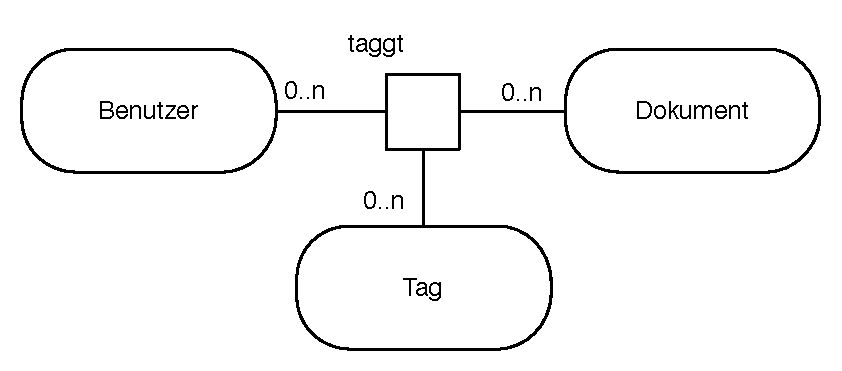
\includegraphics[width=0.75\textwidth]{tag_system}
\caption{FMC--Entity--Relationship--Diagramm eines Tagging--Systems}
\label{fig:tagging_erd}
\end{figure}

Das beschriebene Tagging--System lässt sich somit in ein Datenmodell mit den Entitätstypen \emph{Benutzer}, \emph{Dokument}, \emph{Tag} und  der ternären Beziehung \emph{Tagging} überführen. Dieses Modell ist in \cref{fig:tagging_erd} als Entity--Relationship--Diagramm dargestellt. Alle genannten Entitätstypen können weitere Attribute besitzen, die von der Anwendungsdomäne des konkret betrachteten Tagging--Systems abhängen.

\subsection{Arten von Tagging--Systemen}
\label{tagging_types}

Abhängig vom gewünschten Einsatzzweck des Tagging--Systems kann der Betreiber bestimmte Aspekte des Systems beschränken. Außerdem können die Benutzer einen vorherrschenden Umgang mit dem System entwickeln. Aus diesen Faktoren ergeben sich verschiedene Arten und Nutzungsmuster von Tagging-Systemen. Hauptsächlich kann zwischen offenen Tagging--Systemen, den so genannten \emph{Folksonomies} und den geschlossenen Tagging--Systemen unterschieden werden.

\subsubsection{Folksonomies}

Eine Folksonomy beschreibt ein weitestgehend offenes Tagging--System \cite{ma2004}. Bei dieser Art von System kann grundsätzlich jeder Benutzer jeden Tag an jedes Dokument vergeben. Außerdem stammen die Dokumente selbst meist ebenfalls von den Benutzern. Beispiele für Folksonomies sind der Bookmarking--Dienst \emph{Delicious} \cite{deli} und die Foto-Plattform \emph{Flickr} \cite{flickr}.

Der Begriff \emph{Folksonomy} steht im Gegensatz zur \emph{Taxonomie} und beschreibt den Umstand, dass die Kategorisierung und Ordnung von Inhalten vom \emph{folk}, also den Benutzern selbst vorgenommen werden \cite{vt2007}.

\subsubsection{Geschlossene Tagging--Systeme}

In geschlossenen Tagging--Systemen beschränkt der Betreiber des Systems bestimmte Aspekte. Dies können die Benutzer, die Tags vergeben dürfen, die Dokumente oder auch das Vokabular sein.

Eine häufige Form der Einschränkung, der auch das in dieser Arbeit verwendete System unterliegt (siehe \cref{tag_sprd}), ist die Einschränkung der Benutzer die ein Dokument taggen können. Oftmals ist dies nur den Autoren des Dokumentes selbst oder Benutzern mit besonderen Rechten, beispielsweise Moderatoren oder Angestellten des Betreibers, erlaubt.

In den meisten Tagging--Systemen stammen die Dokumente ebenfalls von den Benutzern des Systems, beispielsweise Artikel, Fotos oder Musikstücke. Jedoch kann die Erstellung der Dokumente eingeschränkt werden, wenn dies in der Anwendungsdomäne sinnvoll ist. Beispiele hierfür sind Produkte in Online--Shops. Diese werden nicht von den Benutzern erstellt, jedoch kann die Vergabe von Tags an diese einen Mehrwert liefern.

Die Einschränkung des Vokabulars kann vorgenommen werden, um Rechtschreibfehler und Fehleingaben der Tags zu vermeiden. Sie bringt jedoch den Nachteil mit sich, dass die Tags dann unter Umständen nicht mehr das Vokabular der Benutzer widerspiegeln und somit Inhalte für diese schwerer auffindbar sind.

\section{Tagging--System von Spreadshirt}

Nachdem im vorherigen Abschnitt die Grundlagen von Tagging--Systemen diskutiert wurden, beschäftigt sich dieser Abschnitt mit dem konkreten Tagging--Systems der Website \emph{Spreadshirt}, welches in dieser Arbeit für den initialen Schritt der Link Discovery genutzt wurde (siehe \cref{ld_tags}).

\subsection{Spreadshirt}
\label{spreadshirt}

Die vorliegende Masterarbeit wurde im Kontext der sprd.net AG (Spreadshirt) \cite{sprd2013} erstellt. Spreadshirt ist eine E--Commerce--Plattform, die es seinen Benutzern erlaubt, personalisierte Textilien und andere Artikel zu gestalten, zu kaufen und zum Verkauf anzubieten. Spreadshirt übernimmt die Produktion und den Versand der Produkte. Ein Produkt bezeichnet hierbei einen Produkttyp, beispielsweise ein T--Shirt, der mit einem oder mehreren Designs bedruckt wurde.

Das Erstellen von Designs und die Konfiguration eines Produktes, also das Positionieren von Designs auf Produkttypen, wird vollständig vom Benutzer durchgeführt. Es agieren grundsätzlich zwei Arten von Benutzern mit der Spreadshirt--Plattform: \emph{Kunden} und \emph{Partner}.

Als Kunden werden Benutzer bezeichnet, die Produkte bestellen. Diese Produkte können entweder von ihnen selbst oder von einem Partner erstellt worden sein. 

Partner sind Benutzer, die Designs oder Produkte erstellen und diese zum Verkauf anbieten. Zu diesem Zweck kann der Partner einen eigenen Shop auf der Spreadshirt--Plattform eröffnen. Kunden können in diesem Shop Produkte bestellen und der Partner erhält einen Anteil des Verkaufspreises, während Spreadshirt die Produktion und den Versand an den Kunden übernimmt.

Neben den von Kunden für sich selbst erstellten Produkten und den Partner--Shops existiert mit dem Spreadshirt--Marktplatz ein weiterer Vertriebskanal. Auf dem Marktplatz können Partner nach ihrer Zustimmung ihre Designs vertreiben. Kunden können nach Motiven suchen, die ihrem Geschmack entsprechen und diese bestellen, mit anderen Motiven kombinieren oder mit Texten versehen. Ein Produkt, das entweder in einem Partner--Shop oder auf dem Marktplatz positioniert und mit einem Preis versehen wurde, wird Artikel genannt.

\begin{figure}[t]
\centering
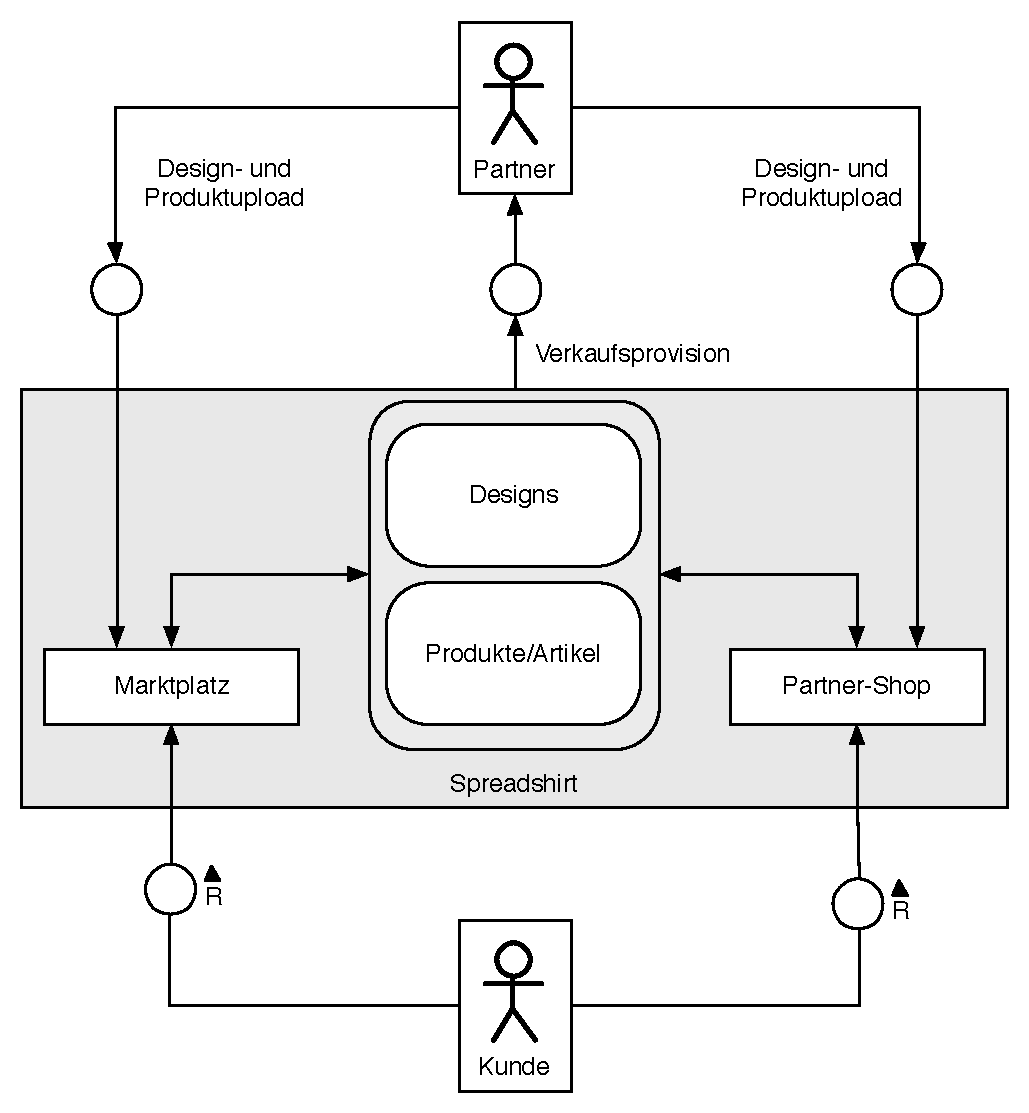
\includegraphics[width=0.65\textwidth]{how_spreadshirt_works}
\caption{FMC--Blockdiagramm der Spreadshirt--Bereiche und Benutzer}
\label{fig:howspreadshirtworks}
\end{figure}

Die grundsätzliche Funktionsweise der Spreadshirt--Plattform ist in \cref{fig:howspreadshirtworks} als FMC--Blockdiagramm dargestellt.

Das Suchergebnis für Suchen auf dem Marktplatz hängt maßgeblich von den Metadaten ab, die der Partner für seine Designs vergeben hat. Dazu gehören Tags, aber auch Titel und Beschreibung des Designs oder Produktes. In dieser Arbeit wird ausschließlich das Tagging--System betrachtet.

\label{platforms}
Spreadshirt betreibt aus historischen Gründen zwei Plattformen, deren Datenbestände größtenteils voneinander getrennt sind. Jeweils eine Plattform ist für den nordamerikanischen und den europäischen Markt zuständig. Im Kontext dieser Arbeit wird die europäische Plattform als Ausgangsbasis für alle Betrachtungen gewählt. Der Datenbestand dieser Plattform besteht aus circa 2 Millionen Tags, 6 Millionen Designs, 14 Millionen Produkten, 6 Millionen registrierten Nutzern und \num{750000} eröffneten Partner--Shops.

\subsection{Eigenschaften des Tagging--Systems}
\label{tag_sprd}

Im Fall von Spreadshirt ist die Vergabe von Tags auf die Menge der Partner \(P \subseteq U\) begrenzt (siehe auch \cref{spreadshirt}). Es handelt sich demnach um ein in \cref{tagging_types} beschriebenes geschlossenes Tagging--System.

Die Dokumente, die von den Partnern getaggt werden können, sind auf die Designs und Artikel beschränkt, die der Partner selbst angelegt hat. Eine Beschreibung kann somit ausschließlich durch den Autor des Inhaltes erfolgen. Deshalb fehlt im Vergleich zu anderen Tagging--Systemen auch die Information, welcher Benutzer den Tag vergeben hat, da diese implizit durch den Autor des Dokumentes gegeben ist.

Des Weiteren besitzen Tags in der Spreadshirt--Datenbank ein Attribut \emph{Sprache} aus der Menge \(L\). Die Sprache spielt bei der Eingabe und Anzeige der Tags zu Dokumenten eine Rolle. Je nach eingestellter Sprache auf der Website erstellt und sieht der Benutzer nur Tags, die mit dieser Sprache markiert sind.

Das Vokabular der Tags ist nicht eingeschränkt. Dies bringt zwangsläufig Probleme der Datenqualität mit sich, welche im folgenden Abschnitt erläutert werden.

\subsection{Datenqualität des Tagging--Systems}
\label{quality}

Die Qualität von Daten wird im Allgemeinen unter mehreren Gesichtspunkten beurteilt. Dazu gehören unter anderem \emph{Korrektheit}, \emph{Vollständigkeit}, und \emph{Redundanzfreiheit} \cite[S. 84 f.]{hkp2012}. Nachfolgend werden die bei Spreadshirt vorhandenen Tagging--Daten nach diesen Kriterien betrachtet und die Quellen eventueller Fehler \cite[S. 43 f.]{jo2003} diskutiert.

\subsubsection{Korrektheit}

Die Korrektheit der Tagging--Daten kann an vielen Punkten angezweifelt werden. Das hervorstechende Problem hierbei ist das Auftreten von Spam. Viele Partner versehen ihre Artikel und Designs mit Tags, die nicht den Inhalt beschreiben. Partner versehen ihre Designs und Artikel mit falschen Tags, damit diese bei populären Suchbegriffen gefunden werden.

Ein weiterer Defekt ist die Inkorrektheit des Attributes \emph{Sprache} der Tags. Die Sprache wird aus der Domain abgeleitet, die der Benutzer, der den Tag eingegeben hat, besucht hat. Viele Partner geben jedoch ihre Tags in mehreren Sprachen ein, um ihre Inhalte besser auffindbar zu machen. Dies führt in der Konsequenz dazu, dass das Attribut Sprache in einem nicht unwesentlichen Teil der Tags als falsch angesehen werden kann.

Die Quelle beider Fehler ist die bewusste Falscheingabe von Informationen, um einen persönlichen Vorteil zu erlangen, da die Partner versuchen, ihre Produkte möglichst zu vielen Sucheingaben in den Ergebnissen auftauchen zu lassen.
                                                                                                                                                                                                                                                                                                                                                                                                              
\subsubsection{Vollständigkeit}

Wie bereits in \cref{tag_sprd} beschrieben, fehlt in den Daten des Spreadshirt--Systems die Angabe, welcher Benutzer einen Tag vergeben hat. Außerdem besitzen die Taggings keinen Zeitstempel. Dies führt in der Konsequenz dazu, dass Spam schwerer erkannt werden kann. Zwar ist bekannt, wann ein Tag das erste Mal verwendet wurde, alle weiteren Verwendungen des Tags haben jedoch keinen Zeitstempel. Der Benutzer, der den Tag angelegt und verwendet hat, kann nur daraus abgeleitet werden, wer den getaggten Artikel angelegt hat.

Die Unvollständigkeit der Daten rührt in erster Linie daher, dass zum Zeitpunkt der Implementierung des Tagging--Systems noch nicht bedacht wurde, dass die fehlenden Attribute später nützlich sein können.

\subsubsection{Redundanzfreiheit}

Bedingt durch die Form der Dateneingabe besteht für das Vokabular des Tag--Systems ein großes Potential für redundante Daten. Da eingegebene Tags durch einen Separator getrennt eingegeben werden müssen, besteht hier Potential zur Fehleingabe. Wird der falsche Separator verwendet, werden die eigentlich getrennten Tags als eine einzige Entität abgespeichert.

Technisch kann jeder Tag genau ein Mal in der Datenbank vorkommen. Jedoch führen Tipp-- und Rechtschreibfehler, unterschiedliche Groß- und Kleinschreibung, verschiedene Arten zusammengesetzte Wörter zu schreiben, Leerräume vor, nach und zwischen Wörtern eines Tags und Tippfehler dazu, dass das gleiche Wort mehrfach in der Datenbank gespeichert wurde.

Außerdem führten in der Vergangenheit Systemfehler und Implementierungsfehler dazu, dass falsche, nicht druckbare Zeichen in den Tags enthalten waren. Nach Beseitigung der Fehler blieben die fehlerhaften Tags bestehen, so dass bei einer erneuten Eingabe des gleichen Wortes ein neuer Tag in der Datenbank angelegt wurde.

\subsection{Mengengerüst des Tagging--Systems}
\label{tag_amount}

Zum Zeitpunkt der Bearbeitung dieser Arbeit befanden sich im Datenbestand der europäischen Spreadshirt--Plattform:

\begin{itemize}
    \item \num{2072079} Tags in \num{15} verschiedenen Sprachen
    \item \num{6433410} Benutzer
    \item \num{26147860} Dokumente (\num{16494430} Artikel und \num{9653430} Designs)
    \item \num{71938905} Taggings
\end{itemize}

Diese Datenmengen stellen besondere Anforderungen an die Verarbeitung. Wie diese umgesetzt wurden, wird in \cref{system} diskutiert.

\section{Zusammenfassung}

Dieses Kapitel befasste sich mit Tagging--Systemen. Dazu wurden die Grundlagen und Begriffe genannt, die Vor-- und Nachteile von Tagging--System erläutert, das Datenmodell formalisiert und die grundsätzlichen Arten Folksonomy und geschlossenes Tagging--System unterschieden.

Außerdem wurde das im weiteren Verlauf dieser Arbeit verwendete Tagging--System von Spreadshirt \cite{sprd2013} näher betrachtet. Dazu wurden die speziellen Eigenschaften dieses Systems, die Datenqualität und die Menge der vorhandenen Daten beschrieben.

Das nachfolgende Kapitel beschäftigt sich mit dem zur Link Discovery angewandten Framework.
\chapter{Link--Discovery--Framework}

\section{Modell des Weltausschnittes}
\label{world_model}

Der folgende Abschnitt beschäftigt sich mit der Modellierung des im Rahmen dieser Arbeit verwendeten Weltausschnittes. 

\begin{figure}
\centering
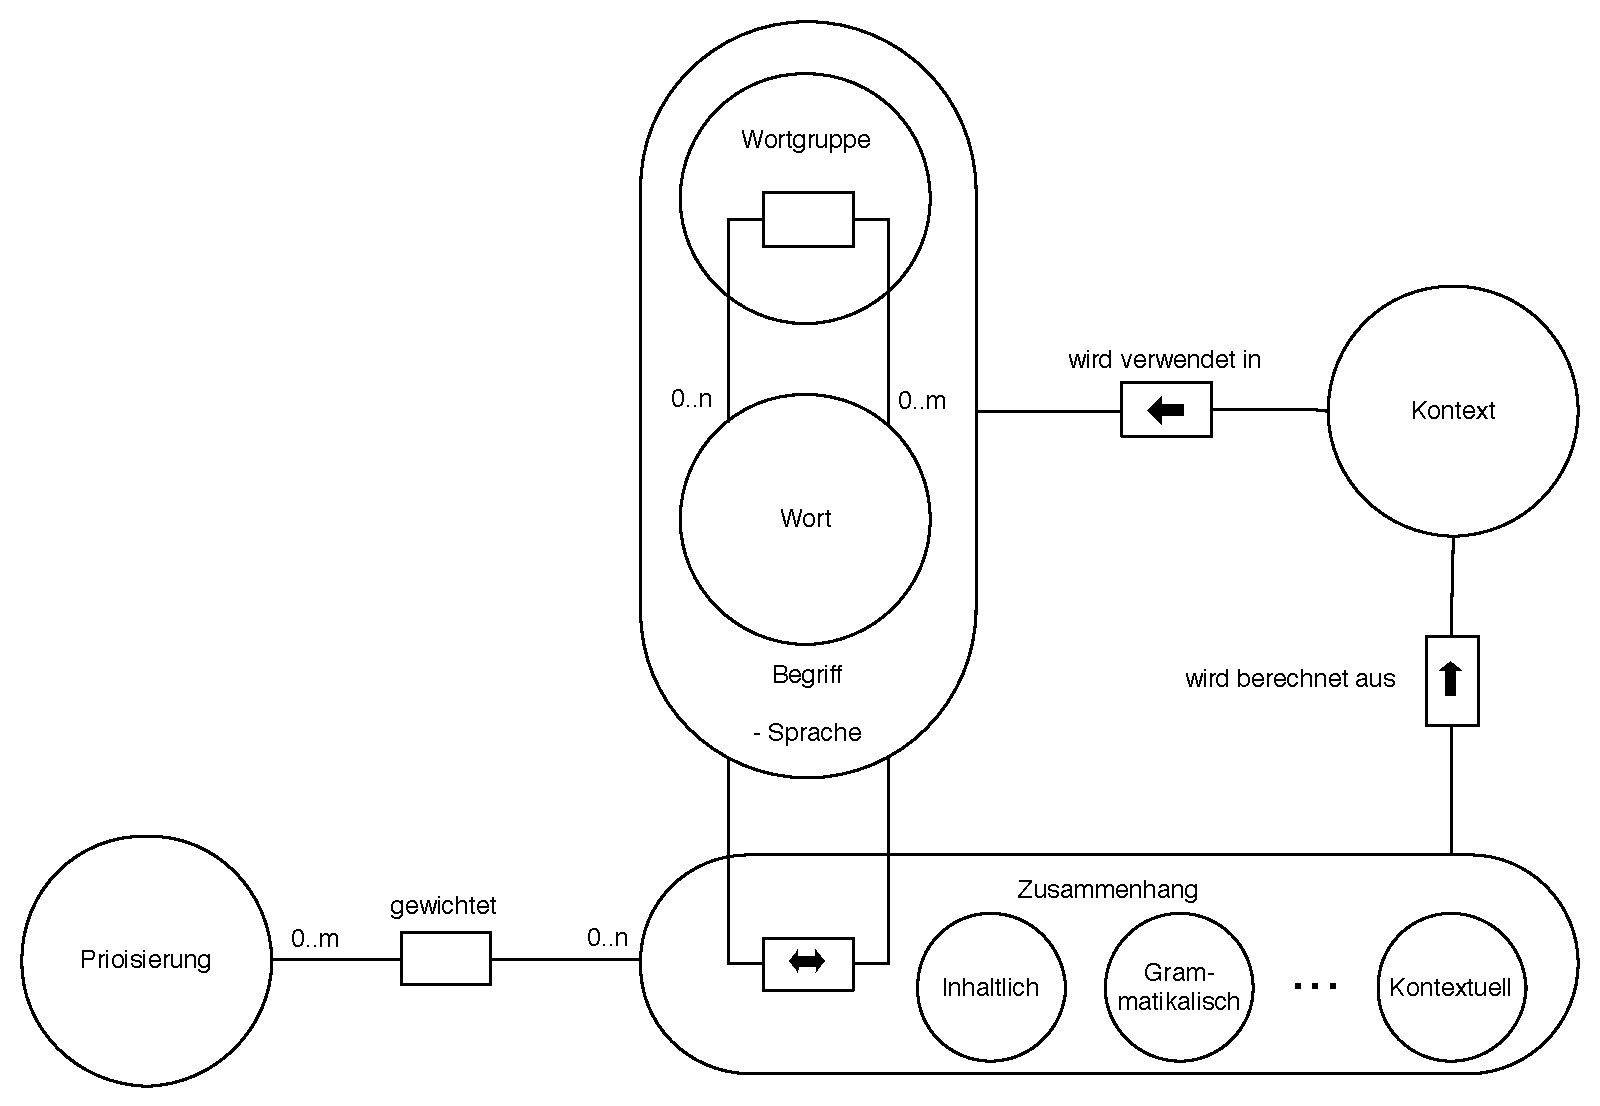
\includegraphics[width=\textwidth]{abstract_world_model}
\caption{Abstraktes Modell des Weltausschnittes}
\label{fig:world_model}
\end{figure}

Abbildung \ref{fig:world_model} zeigt das Modell als Entity--Relationship--Diagramm.

Zentrale Entität ist des Modelles der \emph{Begriff}. Ein Begriff repräsentiert ein Einzelwort oder eine Wortgruppe in einer bestimmten Sprache. Dies berücksichtigt den Umstand, dass Wörter in mehreren Sprachen vorkommen können, jedoch verschiedene Bedeutungen besitzen können. Wortgruppen können aus beliebig vielen Einzelwörtern zusammengesetzt sein. Mit Hilfe der Link Discovery sollen zwischen diesen Begriffen verschiedenartige \emph{Zusammenhänge} gefunden werden.

Ein Zusammenhang besteht immer zwischen genau zwei Begriffen und besitzt einen bestimmten \emph{Typ}. Der Typ bezeichnet die Art des Zusammenhangs zwischen diesen beiden Begriffen. Beispiele für Zusammenhangsarten sind inhaltliche Zusammenhänge wie Synonyme, grammatikalische Zusammenhänge wie Wortformen und Grundformen oder kontextuelle Zusammenhänge, die sich aus der Verwendung des Begriffes ergeben. Dabei kann ein Zusammenhang abhängig vom Typ Attribute besitzen, die den Zusammenhang genauer spezifizieren. Dies kann beispielsweise ein Gewicht des Zusammenhangs sein, dass die Wichtigkeit gegenüber anderen Beziehungen gleichen Typs angibt.

Je nach Nutzungsform der Daten wird unter Umständen eine andere Sicht auf die Beziehungen benötigt. Eine \emph{Prioisierung} stellt eine Gewichtung der Beziehungen eines Begriffes nach Typ dar. Sie teilt jeder Zusammenhangsart ein Gewicht relativ zu den anderen Arten zu. Somit werden durch die Prioisierung bestimmte Zusammenhänge höher gewichtet als andere. Die Prioisierung wird zu einer auf den Anwendungsfall abgestimmten Ordnung der Beziehungen eines Begriffes genutzt.

Dies Verwendung eines Begriffes wird durch den \emph{Kontext} beschrieben. Dieser Kontext repräsentiert, \emph{wo}, \emph{wie} und \emph{wann} der Begriff innerhalb einer bestimmten Anwendungsdomäne verwendet wurde. Daher sind die Attribute, die ein Kontext besitzen kann, nicht vorab spezifizierbar. Sie hängen von der jeweiligen Anwendungsdomäne ab. Beispiele für Kontexte sind die Verwendung eines Begriffes in einem Tag-System oder in einer Ontologie.

Dieses Modell bildet die Grundlage für  im folgenden Abschnitt beschriebenen Link--Discovery--Prozess.

\section{Link--Discovery--Prozess}
\label{ld_process}

Der Link--Discovery--Prozess beschreibt die Abfolge von Schritten, die zur Erzeugung und Anreicherung des in \ref{world_model} beschriebenen Weltausschnittes angewendet werden. Dieser Prozess dient also zur Erzeugung von Begriffen und deren Zusammenhängen. Abbildung \ref{fig:link_discovery_process} zeigt den Prozess als Petrinetz.

\begin{figure}
\centering
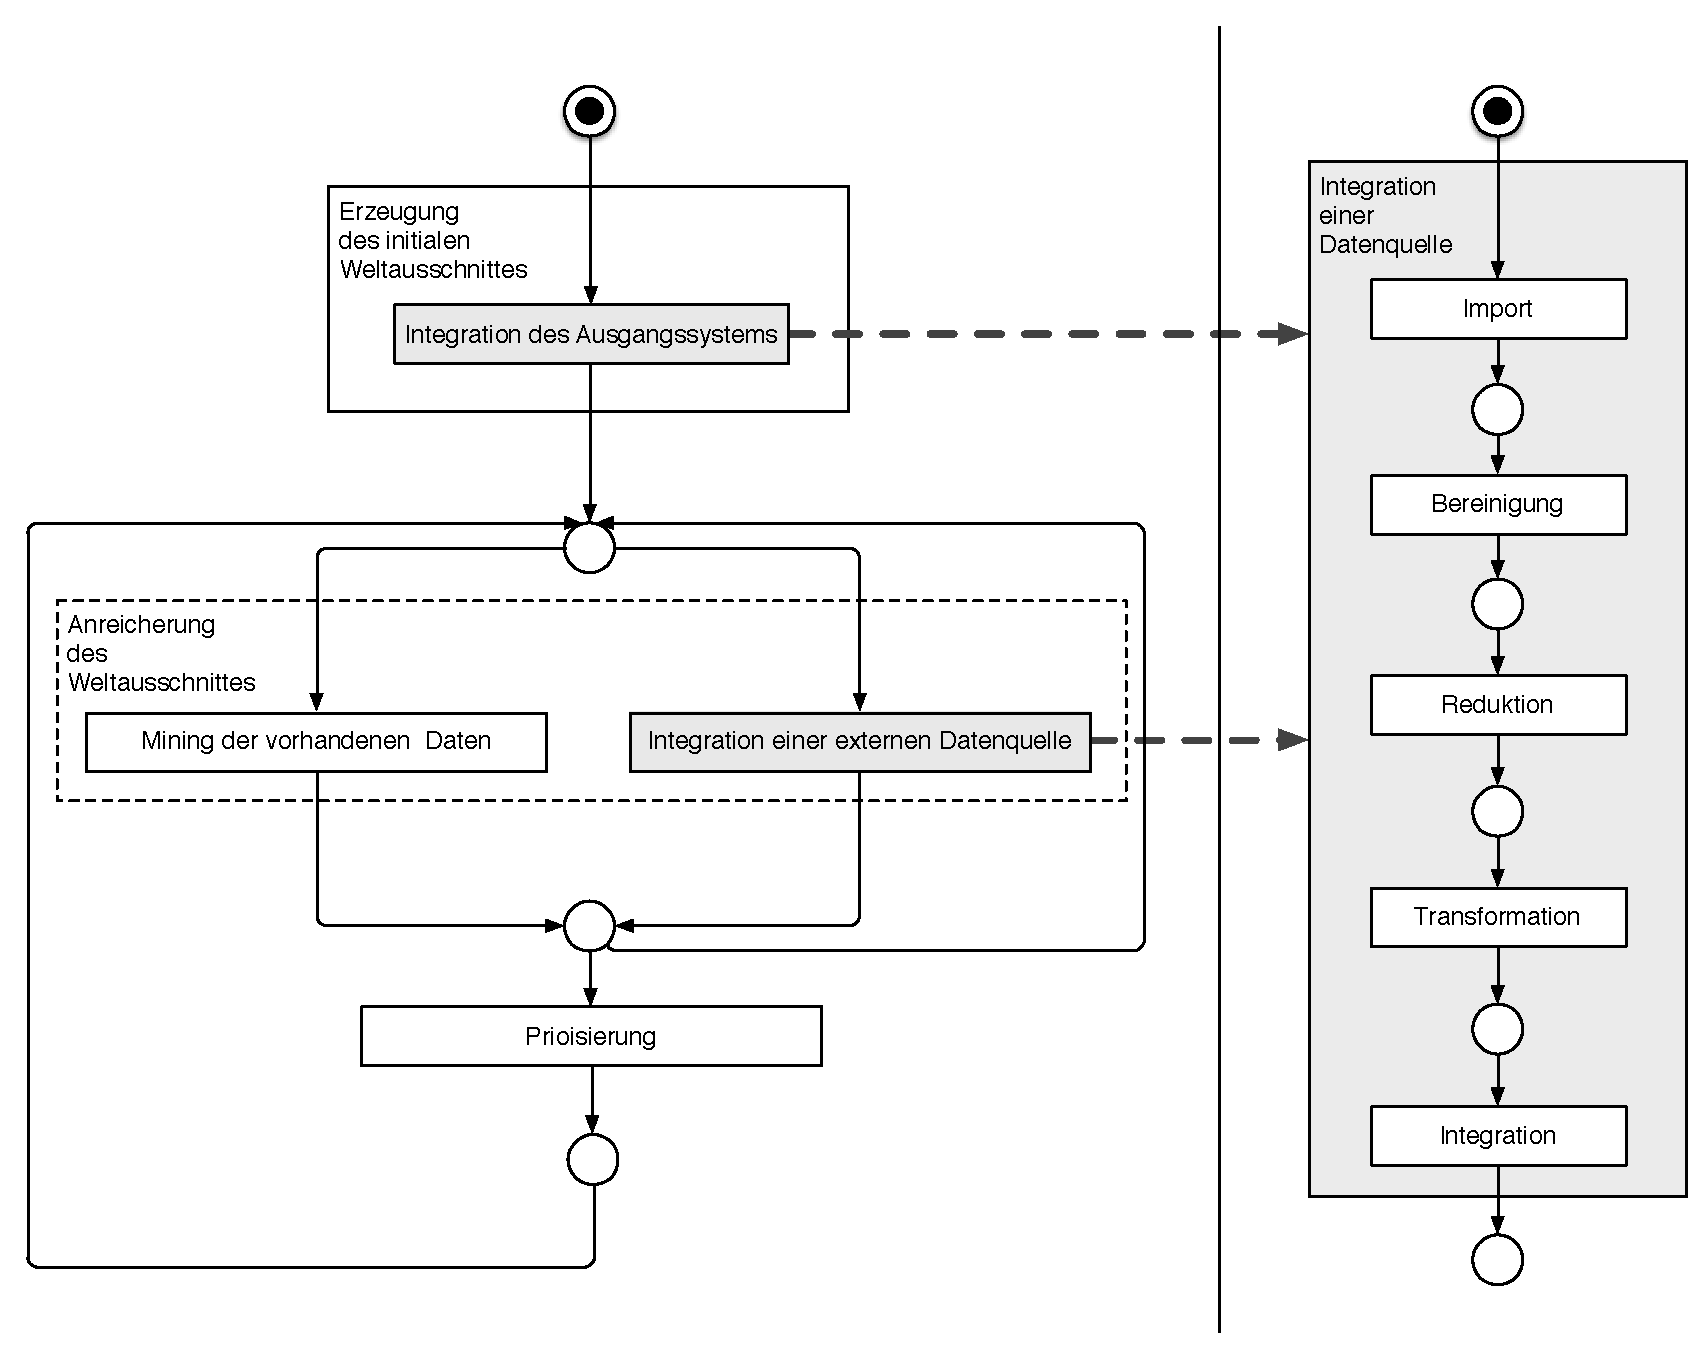
\includegraphics[width=\textwidth]{link_discovery_process}
\caption{Link--Discovery--Prozess als Petrinetz}
\label{fig:link_discovery_process}
\end{figure}

Die grundlegenden Phasen des Prozesses sind die \emph{Erzeugung} des initialen Weltausschnittes, dessen \emph{Anreicherung} und die \emph{Prioisierung} der Beziehungen. Sowohl bei der initialen Erzeugung, als auch bei der Anreicherung wird ein Prozess zur Integration von Datenquellen benötigt.

Die Schritte der Anreicherung und Priosierung können beliebig oft wiederholt werden, um das Ergebnis zu verbessern und auf die gewünschte Anwendung anzupassen. Die Anreicherung kann grundsätzlich durch das Mining der bereits im Weltausschnitt vorhandenen Daten oder durch die Integration neuer Datenquellen erfolgen.

Die genannten Schritte werden in den folgenden Abschnitten erläutert.

\subsection{Integration von Datenquellen}
\label{integration_generic}

Für die Link Discovery wird ein einheitliches Vorgehen zur Integration von Datenquellen benötigt. Die Datenquellen stellen grundsätzlich für die Link Discovery nützliche Daten zur Verfügung, die jedoch im Allgemeinen noch nicht direkt dem Modell des Weltausschnittes entsprechen. Demzufolge müssen diese Daten entsprechend vorverarbeitet werden.

Die zur Integration von externen Datenquellen nötigen Schritte entsprechen im Wesentlichen den von \textcite[S. 48f.]{hkp2012} beschriebenen Aufgaben der Datenvorverarbeitung: \emph{Bereinigung}, \emph{Reduktion}, \emph{Transformation} und \emph{Integration}. Diesen wird in dieser Arbeit der Schritt \emph{Import} vorangestellt, da es nicht immer möglich ist, den gesamten Datenbestand einer Datenquelle zu nutzen. Somit sollten im Importschritt auch die Anfragen an die Datenquelle spezifiziert werden. Die genannten Schritte werden zur Link Discovery immer in der genannten Reihenfolge ausgeführt und werden im folgenden kurz beschrieben.

\paragraph{Import}

Im Importschritt werden die Rohdaten aus der Datenquelle extrahiert. Dabei wird die Form der Daten nicht verändert. Ist es nicht möglich, den gesamten Datenbestand einer Quelle zu importieren, so muss eine Auswahl der anzufragenden Daten formuliert werden. Diese Auswahl richtet sich nach Möglichkeit nach den bereits im Weltausschnitt vorhandenen Daten.

\paragraph{Bereinigung}

Im nachfolgenden Bereinigungsschritt werden die importierten Daten so gut wie möglich von eventuell vorhandenen Defekten bezüglich der Datenqualität (siehe auch \ref{quality}) befreit. Dazu zählen beispielsweise das Entfernen nicht nutzbarer Zeichen oder von unvollständigen Datensätzen.

\paragraph{Reduktion}

Der Reduktionsschritt dient zur Verkleinerung der Datenmenge. Dazu gehören beispielsweise Schritte zur Duplikatentfernung oder zur Auswahl relevanter Datensätze. In dieser Arbeit bestand die Haupteinschränkung der Datenmenge darin, nach Möglichkeit nur deutschsprachige Datensätze auszuwählen.

\paragraph{Transformation}

Der Schritt der Transformation überführt die Daten schließlich in das Modell des Weltausschnittes. Dies bedeutet, dass die Datensätze in Begriffe und Beziehungen umgewandelt werden. Dabei sollten so viele Informationen über den Kontext der Begriffe erhalten bleiben. Die Methode, wie diese Transformation vorgenommen wird, hängt von der Datenquelle ab. Generell werden die Beziehungen meist aus dem Kontext der Begriffe, wie er in der Datenquelle vorliegt, gebildet. Somit stellt der Transformationsschritt die wichtigste Komponente für die Integration einer Datenquelle dar.

\paragraph{Integration}

Der Integrationsschritt für jede Datenquelle dient letztendlich der Zusammenführung des im Transformationsschritt erzeugten Weltausschnittes mit dem bereits vorhandenen Weltausschnitt. Dabei werden bereits existierende Begriffe zusammengeführt und die neu erzeugten Beziehungen übernommen. Die Zusammenführung der Begriffe erfolgt über die Annotation des existierenden Begriffes mit dem neu erzeugten Kontext, den die Datenquelle zu einem Begriff liefert.

\subsection{Initiale Erzeugung des Weltausschnittes}

Der erste Schritt der Link Discovery besteht in der Auswahl einer geeigneten Datenquelle für die initiale Erzeugung des Weltausschnittes. In dieser Arbeit ist diese Datenquelle das Tagging-System von Spreadshirt (siehe \ref{tag_sprd}).

Die Auswahl der Datenquelle richtet sich im wesentlichen danach, ob der Kontext, den die Datenquelle potentiell zu Begriffen liefern kann, für die Link Discovery geeignet ist. Der Kontext sollte außerdem für die geplante Anwendung der Link--Discovery--Ergebnisse relevant sein.

Nach der Auswahl einer geeigneten Quelle werden die in Abschnitt \ref{integration_generic} beschriebenen Schritte zur Integration durchgeführt. Der letzte Schritt ist trivial, da zu diesem Zeitpunkt noch keine Daten vorhanden sind.

\subsection{Anreicherung des Weltausschnittes}

\subsubsection{Anreicherung durch Mining vorhandener Daten}

\subsubsection{Anreicherung durch Integration externer Datenquellen}

\subsection{Priorisierung von Beziehungen}
\include{application}
\chapter{Link--Discovery--System}
\label{system}

Das folgende Kapitel beschäftigt sich mit ausgewählten Aspekten der technischen Umsetzung der in \cref{link_discovery} beschriebenen Link--Discovery--Durchführung. Dazu gehören die Formulierung der Anforderungen an das System, die Systemarchitektur sowie die getroffene Technologieauswahl und einige Implementierungsaspekte.

\section{Anforderungen an das System}
\label{requirements}

Dieser Abschnitt formuliert die Anforderungen an ein System, das zur Link Discovery eingesetzt werden kann. Die Anforderungen unterteilen sich hierbei in einen funktionalen und einen nichtfunktionalen Anteil. 

\subsection{Funktionale Anforderungen}

Nachfolgend werden die funktionalen Anforderungen an das System aufgeführt. Diese ergeben sich direkt aus dem in \cref{ld_framework} beschriebenen Link--Discovery--Framework.

\paragraph{Datenimport} Das System muss in der Lage sein, Rohdaten aus verschiedenen Datenquellen zu importieren und zu speichern. Dazu zählen die MySQL--Datenbank von Spreadshirt, die JSON--Dokumente des Clicktracking--Systems und die API des Wortschatzes der Universität Leipzig. Das System sollte außerdem erweiterbar sein, um in Zukunft andere Datenquellen einbinden zu können.

\paragraph{Datenspeicherung} Das System muss die importierten Rohdaten, Zwischenergebnisse der Link Discovery und die Graphenrepräsentation des Weltausschnittes permanent speichern können.

\paragraph{Datenverarbeitung} Das System muss die importierten Daten entsprechend des in \cref{ld_process} beschriebenen Link--Discovery--Prozesses verarbeiten können. Dazu zählen die Schritte Bereinigung, Reduktion, Transformation und Integration. Die Implementierung dieser Schritte sollte änderbar und erweiterbar sein. Im Rahmen des Transformationsschrittes muss das System in der Lage sein, Kookkurrenzmaße zu berechnen.

\paragraph{Visualisierung} Das System soll eine Oberfläche für die Visualisierung der in der Graphenrepräsentation des Weltausschnittes gespeicherten Daten bieten. Dazu zählen die Darstellung der Begriffe, deren Kontext und Beziehungen und eine Möglichkeit der manuellen Priorisierung zum interaktiven Erkunden des Datenbestandes.

\paragraph{Priorisierung} Das System muss den in \cref{evo_for_prio} beschriebenen Priorisierungsprozess mittels evolutionärer Algorithmen implementieren. Dazu gehören Komponenten des Algorithmus aus \cref{evo_implementation} sowie eine Benutzeroberfläche zur interaktiven Selektion.

\paragraph{Programmierschnittstelle} Das System muss eine Programmierschnittstelle (im Folgenden \emph{API}) zur programmatischen Abfrage der Daten bereit stellen. Die angebotenen Daten enthalten die Begriffe, deren Kontexte und priorisierte Beziehungen. Die Priorisierung wird vom Benutzer der API spezifiziert.

\subsection{Nichtfunktionale Anforderungen}

Neben den funktionalen Anforderungen werden einige nichtfunktionale Anforderungen an das System gestellt. Diese werden im folgenden genannt.

\paragraph{Datenmenge} Das System muss in der Lage sein, bis zu einer Milliarde Objekte zu speichern und zu verarbeiten. Diese Objekte können Rohdaten der Datenquellen, Zwischenergebnisse der Link Discovery oder Knoten und Kanten des Weltausschnittes sein.

\paragraph{Parallelisierbarkeit} Um die Datenmenge verarbeiten zu können, sollten rechenintensive Berechnungsschritte auf mehrere Rechner verteilt werden können, um die Berechnung zu beschleunigen. Zu den anspruchsvolleren Berechnungsschritten zählt beispielsweise die Berechnung von Kookkurrenz aus den Daten des Tagging--Systems.

\paragraph{Antwortzeiten} Das System sollte Anfragen, die die Graphenrepräsentation des Weltausschnittes betreffen, in unter einer Sekunde beantworten. Hierzu zählt vor allem die Anfrage der Nachbarn eines Begriffes, geordnet nach einer spezifizierten Priorisierung.

Nachdem die Anforderungen an das System formuliert wurden, werden in den folgenden Abschnitten die sich daraus ergebende Architektur, das Datenmodell und die Technologieauswahl erläutert.

\section{Architektur des Systems}
\label{architecture}

Aus den im vorherigen Abschnitt formulierten Anforderungen wurde die im Folgenden beschriebene Systemarchitektur entwickelt. \cref{fig:architecture} zeigt die komplette Architektur des implementierten Link--Discovery--Systems. Darin sind, neben der Architektur des Systems selbst, alle genutzten Datenquellen und die Daten, die sie bereit stellen, aufgeführt.

\begin{figure}
\centering
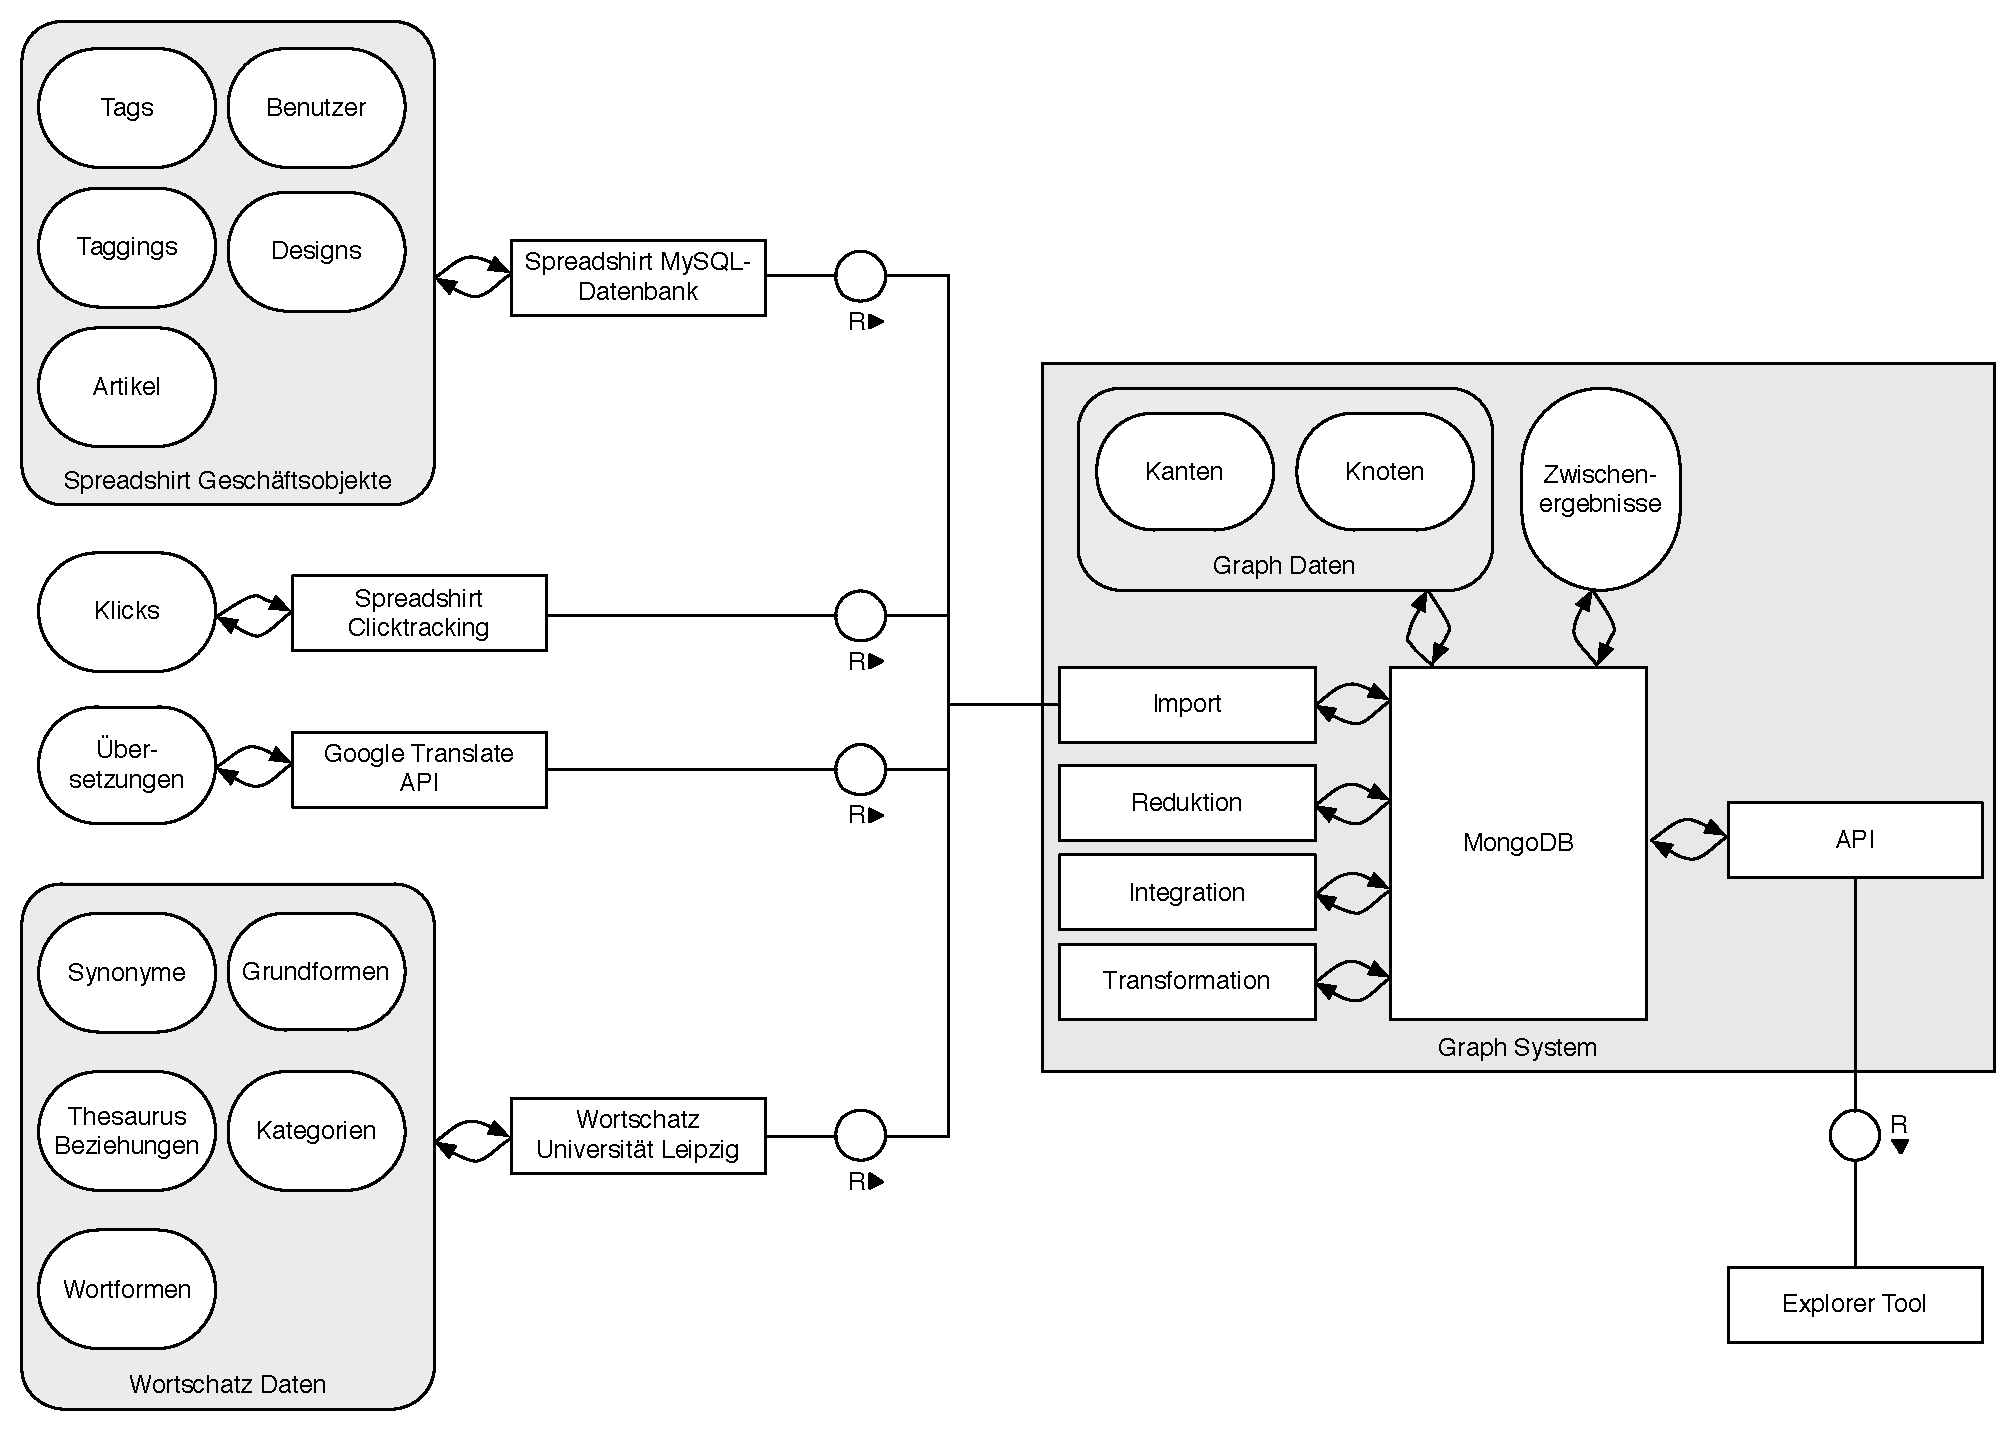
\includegraphics[width=1\textwidth]{architecture}
\caption{FMC--Blockdiagramm der gewählten Systemarchitektur}
\label{fig:architecture}
\end{figure}

Zentraler Bestandteil der Architektur ist das Datenbanksystem, das alle benötigten Daten speichert. Die Wahl des Datenbanksystems hat große Bedeutung für die Realisierung der funktionalen und nichtfunktionalen Anforderungen und wird in \cref{db_choice} diskutiert. Im Datenbanksystem werden die Rohdaten, Zwischenergebnisse und die Graphenrepräsentation des Weltausschnittes abgelegt. Das Datenmodell des Graphen folgt der Definition aus \cref{world_graph}.

Für jeden Schritt der Integration von Datenquellen aus \cref{integration_generic} existiert in der Architektur eine Komponente, die den jeweiligen Schritt für die entsprechende Datenquelle ausführt. Diese Komponenten kommunizieren direkt mit dem Datenbanksystem, um die Rohdaten oder Zwischenergebnisse zu lesen, führen die Berechnungen durch und speichern die Ergebnisse wiederum in die Datenbank.

Für die Abfrage der im Graphen gespeicherten Informationen existiert eine API, welche Informationen zu Knoten und deren Nachbarn per HTTP als JSON--Dokumente \cite{json2006} zur Verfügung stellt. Diese API kann für die Einbindung der erzeugten Informationen in andere Applikationen genutzt werden. Über Anfrageparameter kann die Gewichtung der einzelnen Kantentypen beeinflusst werden.

Zum Zeitpunkt der Bearbeitung dieser Arbeit existierten zwei Anwendungen, die die API des Link--Discovery--Systems nutzten. Dies sind der \emph{Tag Explorer} und die Komponente zur Priorisierung der Beziehungen.

Beim Tag Explorer handelt es sich um eine Browseranwendung, die die im Graphen gespeicherten Beziehungen visualisiert und interaktiv erkundbar macht. Der Benutzer dieser Anwendung kann mit selbst gewählten Gewichtungen der Beziehungen den Graphen durchsuchen. Außerdem werden, wenn vorhanden, die Designs auf der Spreadshirt--Plattform angezeigt, die mit dem gewählten Begriff getaggt sind. Somit wurde die funktionale Anforderung, den Kontext zu einem Begriff zu visualisieren, nur zum Teil umgesetzt, da der Tag Explorer lediglich den Tagging--Kontext eines Begriffes darstellt. In \cref{fig:tag_explorer} ist ein Screenshot der Anwendung abgebildet.

\begin{figure}
\centering
\includegraphics[scale=0.25]{tag_explorer}
\caption{Screenshot der Anwendung ``Tag Explorer''}
\label{fig:tag_explorer}
\end{figure}

Die zweite Anwendung, die die API des Systems nutzt, ist die in \cref{evo_implementation} beschriebene Umsetzung der Priorisierung. Da diese die Daten des Weltausschnittes nicht verändern muss, ist eine entkoppelte Anbindung über die API sinnvoll.

Nachdem die Architektur vorgestellt wurde, spezifiziert der nächste Abschnitt die konkreten Technologien, die zur Implementierung dieser Architektur ausgewählt wurden.

\section{Technologieauswahl}
\label{tech}

Der folgende Abschnitt beschäftigt sich mit einer Auswahl der zur Umsetzung der Link Discovery eingesetzten Technologien. Die Kernelemente sind das Datenbanksystem, die konkrete Implementierung der Architekturkomponenten sowie die Datenverarbeitung mittels des Programmiermodells MapReduce.

\subsection{Datenbanksystem}
\label{db_choice}

Die Wahl des Datenbanksystems ist von zentraler Bedeutung für die Umsetzung der in \cref{requirements} formulierten Anforderungen. Speziell die nichtfunktionalen Anforderungen der großen Datenmenge, der Parallelisierbarkeit und der kurzen Antwortzeiten stellen für traditionelle relationale Datenbanksysteme große Herausforderungen dar. Durch die starre relationale Form der Daten sind Schemaänderungen mit großem Aufwand verbunden. Die Verteilung von Daten über mehrere Server ist üblicherweise nicht grundsätzlich vorgesehen und kann nur mit größerem Implementierungsaufwand erreicht werden. Aufgrund dieser häufigen Limitierungen relationaler Datenbanksysteme wurde für die Implementierung des Link--Discovery--Systems das Datenbanksystem \emph{MongoDB} \cite{mo2013} gewählt.

\subsubsection{MongoDB}
\label{mongo}

Bei MongoDB handelt es sich um eine quelloffene dokumentenorientierte Datenbank. Im Gegensatz zu traditionellen relationalen Datenbanksystemen verzichtet MongoDB auf eine tabellenförmige Struktur der Daten und speichert Datensätze in Form von so genannten \emph{Dokumenten}. Dabei handelt es sich um hierarchische Schlüssel-/Wertpaare, die schemalos in so genannten \emph{Collections} gespeichert werden. Schemalos bedeutet, dass die Dokumente innerhalb einer Collection nicht alle dieselbe Struktur besitzen müssen.

Zur Repräsentation der Dokumente verwendet MongoDB ein Format, das sich sehr an JSON \cite{json2006} anlehnt. JSON ist ein menschenlesbares Datenaustauschformat, das aus der Objektnotation der Programmiersprache JavaScript abgeleitet wurde. Das Datenformat von MongoDB ist BSON \cite{bson2013}, eine binäre Repräsentation von JSON, die einige zusätzliche Datentypen unterstützt. 

\cref{lst:json} zeigt ein Beispiel für ein Dokument in MongoDB. Das Feld \emph{\_id} ist hierbei ein  Bezeichner vom Typ \emph{ObjectID}. Dieser stellt einen global eindeutigen Bezeichner dar, der benutzt werden kann, um Dokumente zu referenzieren. Innerhalb einer Collection muss \emph{\_id} grundsätzlich eindeutig sein. Das Feld \emph{address} zeigt, dass Dokumente weitere Dokumente enthalten können. Am Feld \emph{friends} wird deutlich, dass Werte für Schlüssel auch Arrays von Werten sein können. Diese sind nicht auf primitive Typen wie Zeichenketten oder Zahlen beschränkt, sondern können auch weitere Dokumente oder Arrays sein.

\begin{lstlisting}[language=json, label={lst:json}, caption={JSON--Beispiel für ein Dokument in MongoDB}, float]
{
    "_id" : ObjectId("51efc20147cae77dfc02e0ac"),
    "name" : "Bob",
    "age": 25,
    "address": {
        "city": "Leipzig",
        "street": "Karl--Liebknecht--Str. 132"
        "zip": "04277"
    },
    "friends" : [
        "alice",
        "fred",
        "jason"
    ]
}
\end{lstlisting}

MongoDB unterstützt Anfragen über ein Binärprotokoll, welches über so genannte \emph{Treiber} in vielen Programmiersprachen abstrahiert zur Verfügung steht. Dieses Protokoll unterstützt vielfältige Lese- und Schreiboperationen, die komplexe Abfragen und Operationen auf den gespeicherten Daten zulassen. Außerdem bietet MongoDB eine Implementierung des MapReduce--Programmiermodells (siehe \cref{mapreduce}) sowie die Möglichkeit, Indizes auf allen Hierarchieebenen der Dokumente zu nutzen. Für interaktive Operationen steht die \emph{Mongo Shell} zur Verfügung, welche Abfragen mittels der Programmiersprache JavaScript erlaubt und somit einen Treiber für diese Sprache darstellt.

Aufgrund der genannten Eigenschaften stellt MongoDB einen exzellenten Ausgangspunkt für die Link Discovery im Rahmen dieser Arbeit dar. Durch die vorhandene Schemaflexibilität können die Daten in der gerade benötigten Form gespeichert und abgefragt werden. Durch die Unterstützung von MapReduce mit mehreren Rechnern lassen sich Berechnungen wie die der Kookkurrenz (siehe \cref{mapreduce_cooccurence}) parallelisieren und somit beschleunigen. Die Unterstützung von Indizes auf allen Hierarchieebenen der Dokumente bietet Vorteile zur effektiven Verkürzung von Antwortzeiten auf Anfragen.

MongoDB stellt das zentrale technische Element für die Link Discovery im Rahmen dieser Arbeit dar. Sobald die Daten aus den externen und internen Quellen in MongoDB importiert wurden, können die folgenden Schritte direkt mit Datenbankabfragen realisiert werden.

\subsubsection{Umsetzung der Graphenrepräsentation}

Um das in \cref{world_graph} beschriebene Datenmodell in MongoDB umzusetzen, muss es in eine Dokumentenform überführt werden. Dazu bietet es sich an, Knoten in Kanten in unterschiedlichen Collections zu speichern, um sie voneinander zu trennen.

Somit stellt sich anschließend die Frage, wie die Knoten und Kanten als Dokumente repräsentiert werden. Durch die durch MongoDB gegebene Schemaflexibilität lassen sich die Kontexte der durch die Knoten repräsentierten Begriffe direkt als Unterdokumente im Knotendokument ablegen. Der Schlüssel für diese Unterdokumente ist der Name des Kontextes. Dadurch lassen sich die Knoten leicht filtern, da die Abfrage auf das Vorhandensein des jeweiligen Schlüssels angepasst und durch Indizes auf diesen Schlüsseln unterstützt werden kann. \cref{lst:node_json} zeigt ein Beispiel für einen Knoten in JSON--Notation. Arrays mit vielen Elementen sind aus Platzgründen verkürzt dargestellt.

Die Kanten können direkt als Dokumente abgebildet werden. Über den Typ ergeben sich zusätzliche Eigenschaften. \cref{lst:edge_json} zeigt beispielhaft ein Kantendokument für eine Tagging--Kookkurrenz in JSON--Notation.

\begin{lstlisting}[language=json, label={lst:node_json}, caption={JSON--Beispiel für ein Knotendokument in MongoDB}, float]
{
    "_id" : ObjectId("51efc22447cae77dfc03e16b"),
    "language" : "de",
    "string" : "segeln",
    "tagProperties" : {
        "occurenceCount" : 4678,
        "articleCount" : 2347,
        "designCount" : 2331,
        "articleIDs" : [ 
            4961057, 
            4977725, 
            ...
        ],
        "designIDs" : [ 
            1645572, 
            2216059, 
            ...
        ]
    },
    "wortschatzProperties" : {
        "synonyms" : [ 
            "flattern", 
            "fliegen", 
            "gaukeln", 
            ...
        ]
    }
}
\end{lstlisting}

\begin{lstlisting}[language=json, label={lst:edge_json}, caption={JSON--Beispiel für ein Kantendokument}, float]
{
        "_id" : ObjectId("51efd6f61177ff360605bd99"),
        "source" : ObjectId("51efc1af47cae77dfc00c3f8"),
        "target" : ObjectId("51efc1e047cae77dfc02087c"),
        "type" : "tag-co-occurence",
        "occurences" : 1,
        "dice" : 0.0001317089232795522,
        "jaccard" : 0.00006585879873551106,
        "cosine" : 0.008115343414514944
}
\end{lstlisting}

\subsection{Implementierung der Komponenten der Architektur}
\label{arch_components_impl}

Die Komponenten zum Import, zur Bereinigung, Reduktion, Transformation und Integration wurden in der Programmiersprache JavaScript als Skripte für die Mongo Shell (siehe \cref{mongo}) umgesetzt. Diese Skripte implementieren die funktionalen Anforderungen an das System.

JavaScript wurde ausgewählt, da die Sprache eine natürliche Interaktion mit dem JSON--Format ermöglicht. Die Mongo Shell stellt alle Operationen für MongoDB für diese Programmiersprache zur Verfügung und eignet sich damit gut zur Kommunikation mit dem Datenbanksystem.

Die API wurde ebenfalls in JavaScript programmiert, unter Zuhilfenahme der Laufzeitumgebung \emph{node.js} \cite{node}. Diese ermöglicht die serverseitige Benutzung von JavaScript und ist demnach gut geeignet, um mit den Daten aus MongoDB zu arbeiten und diese als JSON--Dokumente an Clients auszuliefern. Der Tag Explorer sowie die Oberfläche zur interaktiven Selektion sind in JavaScript als Browseranwendungen implementiert.

Einzig die Importskripte für die MySQL--Datenbank von Spreadshirt und den Wortschatz der Universität Leipzig wurden in der Programmiersprache Ruby umgesetzt, da diese zum Zeitpunkt des Imports bessere Unterstützung für diese Datenquellen bot.

Zusammenfassend lässt sich festhalten, dass die Architekturkomponenten größtenteils als Skripte implementiert wurden, die direkt mit MongoDB kommunizieren. Dadurch kann das System bei Benutzung von weiteren Datenquellen einfach erweitert werden.

\subsection{Datenverarbeitung}
\label{mapreduce}

Um die nichtfunktionalen Anforderungen an das Link--Discovery--System umzusetzen, wurde zur Verarbeitung der Daten, speziell zur Kookkurrenzberechnung, das Programmiermodell MapReduce gewählt, da dieses die parallele Verarbeitung großer Datenmengen ermöglicht. Die Grundlagen dieses Modells sowie die Umsetzung der Kookkurrenzberechnung werden in den folgenden Abschnitten beschrieben.

\subsubsection{Grundlagen von MapReduce}
\label{mapreduce_basic}

MapReduce \cite{dg2004} ist ein Programmiermodell für nebenläufige Verarbeitung und Erzeugung großer Datenmengen. Der Grundgedanke dieses Modells besteht in der Zerlegung der Berechnung in zwei Funktionen: \emph{Map} und \emph{Reduce}. Die Ein- und Ausgabedaten sind Schlüssel-/Wertpaare. Beide Funktionen werden vom Benutzer spezifiziert.

Die Map--Funktion dient zur Erzeugung von Zwischenergebnissen, welche ebenfalls in der Form von Schlüssel-/Wertpaaren vorliegen. Die Funktion wird einzeln auf jedes Paar der Eingabedaten angewandt und kann eine beliebige Anzahl von Zwischenergebnissen \emph{emittieren}. Die MapReduce--Bibliothek gruppiert daraufhin alle Paare mit dem gleichen Schlüssel und übergibt diese an die Reduce--Funktion.

Die Reduce--Funktion wird somit jeweils auf einen Schlüssel und eine Liste von Werten angewandt. Ziel dieser Funktion ist, für jeden Schlüssel kein oder ein Ergebnis zurückzugeben. Die zu reduzierenden Werte werden für gewöhnlich als Iterator übergeben, um auch Datenmengen verarbeiten zu können, die nicht in den Arbeitsspeicher des Rechenknotens passen. Die Reduce--Funktion wird nur angewandt, wenn nach dem Map--Schritt mehr als ein Wert für einen Schlüssel emittiert wurde. Somit sollten Map- und Reduce--Funktion das gleiche Ausgabeformat besitzen. Das grundsätzliche Vorgehen von MapReduce ist in \cref{fig:mapreduce} abgebildet.

\begin{figure}
\centering
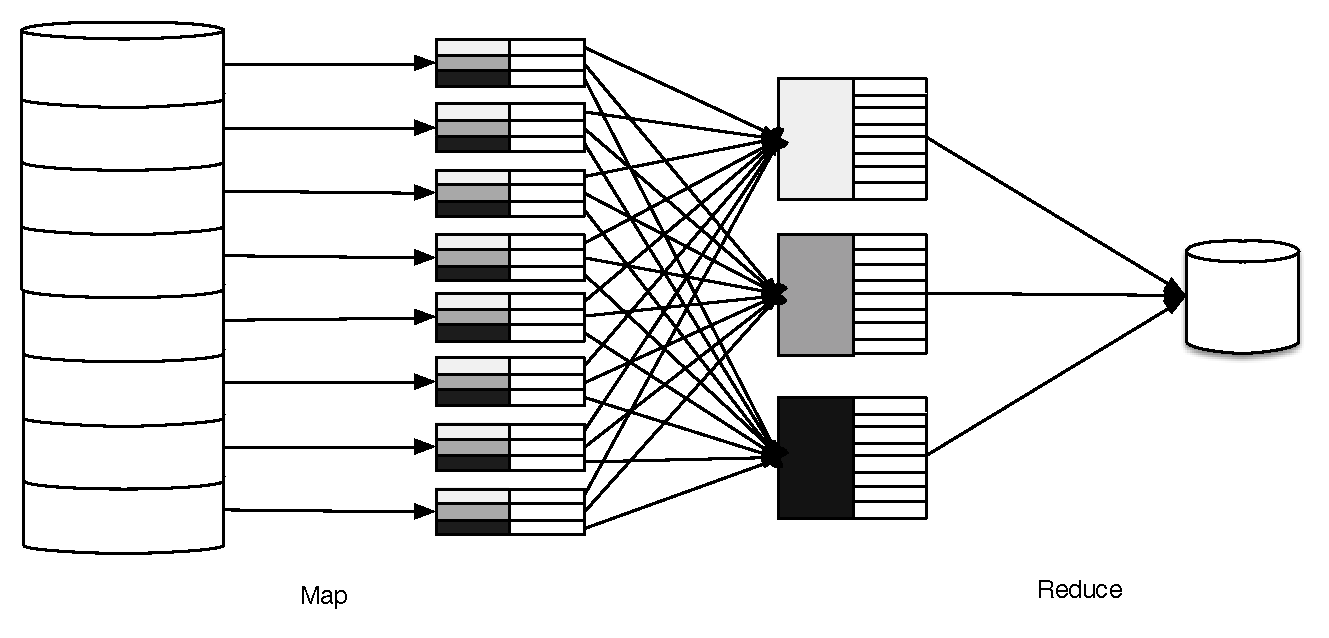
\includegraphics[width=\textwidth]{mapreduce}
\caption{MapReduce--Prozess}
\label{fig:mapreduce}
\end{figure}

Die MapReduce--Bibliothek übernimmt die Kommunikation zwischen den Knoten des Rechnerclusters. Dies hat den Vorteil, dass sich der Programmierer nur über die Umwandlung des zu lösenden Problems auf das Programmiermodell, nicht aber um dessen Implementierung über mehrere Rechner hinweg kümmern muss. Somit kann die verwendete Hardware vergleichsweise einfach an die zu verarbeitende Datenmenge oder die Bedürfnisse an die Rechengeschwindigkeit angepasst werden.

In dieser Arbeit wurde die MapReduce Implementierung von MongoDB eingesetzt (siehe \cref{db_choice}).

\subsubsection{Kookkurrenzberechnung mit MapReduce}
\label{mapreduce_cooccurence}

MapReduce kann für die Berechnung der Knoten und Kanten mittels Kookkurrenz genutzt werden. Dazu müssen für beide Operationen das Ein- und Ausgabeformat sowie die Funktionen Map und Reduce definiert werden.

Um die Berechnung zu vereinfachen, werden zuerst die Knoten erzeugt und mit allen Vorkommen der Begriffe annotiert. Somit kann daraufhin direkt aus der Knotenmenge die Kantenmenge erzeugt werden. Außerdem werden bei der Nutzung der Daten weniger Anfragen benötigt, um Informationen über einen Begriff selbst zu bekommen.

\paragraph{Berechnung der Knoten}

Als Eingabedaten für die Berechnung der Knotenmenge dienen Tupel der Form \((d, t)\), wobei \(d\) ein Dokument und \(t\) einen Begriff darstellt. Die Map--Funktion wird nun auf jeden dieser Tupel angewandt und emittiert Schlüssel-/Wertpaare mit dem Begriff als Schlüssel und einer einelementigen Liste, die das Dokument des Tupels enthält sowie der Zahl \num{1} als Anzahl Vorkommen dieses Begriffs. Dieses Vorgehen ist notwendig, da die Ausgabe der Map- und Reduce--Funktionen das gleiche Datenformat haben sollten.

Die Reduce--Funktion fasst die einelementigen Listen zusammen, addiert die Vorkommen und erzeugt somit den Knoten, der für einen Begriff alle Dokumente, die mit diesem Begriff versehen wurden, sowie die Anzahl der Vorkommen insgesamt enthält.

Die Map- und Reduce--Funktionen für die Knotenberechnung sind in \cref{lst:mapred_nodes} als Pseudo--Code dargestellt.

\begin{lstlisting}[language=pseudo, label={lst:mapred_nodes}, caption={Knotenerzeugung mit MapReduce}, float]
function map(document, term) {
    emit(term, {documents: [document], count: 1});
}

function reduce(term, values) {
    result = {documents: [], count: 0};
    foreach value in values do
        result.documents = concat(result.documents, value.documents);
        result.count = result.count + value.count;
    end
    return result;
}
\end{lstlisting}

\paragraph{Berechnung der Kanten}

Die Berechnung der Kantenmenge kann mit den vorher berechneten Knoten als Eingabedaten erfolgen und wird in 2 Verarbeitungsschritte aufgeteilt. Zuerst werden die annotierten Knoten so umgeformt, dass zu einem Dokument alle vergebenen Begriffe bekannt sind. Im zweiten Schritt werden alle Paare von miteinander auftretenden Begriffen gebildet und die Ähnlichkeitsmaße berechnet.

\cref{lst:mapred_edges1} zeigt die Umformung der Knoten mittels MapReduce. Als Eingabe für die Map--Funktion dienen die Knoten. Diese werden so umgeformt, dass für jedes Dokument, das am Knoten annotiert ist, ein neues Schlüssel-/Wertpaar emittiert wird. Die Reduce--Funktion fasst die emittierten Ergebnisse zusammen, so dass als Ergebnis alle Begriffe, die an ein Dokument vergeben wurden, gesammelt als Liste vorliegen.

\begin{lstlisting}[language=pseudo, label={lst:mapred_edges1}, caption={Umformung der Knoten mit MapReduce}, float]
function map(node) {
    foreach document in node.documents do
        emit(document, {terms: [node]});
    end
}

function reduce(term, values) {
    result = {terms: []};
    foreach value in values do
        result.terms = concat(result.terms, value.terms);
    end
    return result;
}
\end{lstlisting}

In \cref{lst:mapred_edges2} wird die Erzeugung der Kookkurrenzkanten dargestellt. Im Map--Schritt werden dazu alle möglichen Paare der mit einem Dokument verknüpften Begriffe gebildet und emittiert. Der Schlüssel ist eine Kombination aus Ziel- und Quellbegriff. Der Wert zählt die Anzahl der Kookkurrenzen zwischen beiden Begriffen. Während des Reduce--Schrittes werden alle Kanten zwischen zwei Begriffen zusammengefasst, die Summe der Kookkurrenzen gebildet und die Ähnlichkeitsmaße berechnet. Die Funktionen zur Berechnung der Maße sind in \cref{measures} beschrieben.

\begin{lstlisting}[language=pseudo, label={lst:mapred_edges2}, caption={Kantenerzeugung mit MapReduce}, float]
function map(document) {
    foreach term1 in document.terms do
        foreach term2 in document.terms do
            emit({source: term1, target: term2}, {count: 1});
        end
    end
}

function reduce(edge, values) {
    result = {count: 0, dice: 0, jaccard: 0, cosine: 0};
    foreach value in values do
        result.count = result.count + value.count;
    end
    result.dice = dice(edge.source, edge.target, result.count);
    result.jaccard = jaccard(edge.source, edge.target, result.count);
    result.cosine = cosine(edge.source, edge.target, result.count);
    return result;
}
\end{lstlisting}

MapReduce eignet sich somit gut zur Beschleunigung der Kookkurrenzberechnung, da diese in drei Schritten ohne sequenzielle Anteile auf die Funktionen Map und Reduce abgebildet werden kann, wie in diesem Abschnitt gezeigt wurde.

\section{Zusammenfassung}

Dieses Kapitel beschäftigte sich mit den Implementierungsaspekten des Systems, welches für die in \cref{link_discovery} beschriebene Link--Discovery--Durchführung im Rahmen dieser Arbeit zum Einsatz kam. Dazu wurden die funktionalen und nichtfunktionalen Anforderungen an das System formuliert. Aus diesen Anforderungen und dem Prozess zur Link Discovery aus \cref{ld_process} wurde eine Architektur für das System abgeleitet und erläutert. Abschließend wurden einige Technologien, die zur Implementierung des Systems zum Einsatz kamen, diskutiert. Hierzu gehören MongoDB als Datenbanksystem, JavaScript als Sprache für die einzelnen Komponenten der Systemarchitektur und MapReduce als übergeordnetes Programmiermodell sowie dessen konkreter Einsatz zur Kookkurrenzberechnung.
\chapter{Schlussbetrachtung}
\label{summary}

\section{Fazit}

\section{Ausblick}

\cleardoublepage
\pagenumbering{Alph}
\sloppy

\listoffigures
\listoftables
\lstlistoflistings
\printbibliography 

\fussy

\appendix
\chapter{Ergebnisse der Priorisierung}
\label{other_results}

\begin{table}
\centering
\begin{tabular*}{0.9\textwidth}{@{\extracolsep{\fill} } lr}
    \toprule
    Begriff & Gewicht \\
    \midrule
    sex drugs dubstep & \num{0.58} \\
    dubstep beat & \num{0.58} \\
    dubstep music & \num{0.56} \\
    dubstep musik & \num{0.56} \\
    dubstep london & \num{0.56} \\
    \bottomrule
\end{tabular*}
\caption{Nachbarn des Begriffes ``Dubstep'' nach der Priorisierung}
\label{tab:prio_res_dubstep}
\end{table}

\begin{table}
\centering
\begin{tabular*}{0.9\textwidth}{@{\extracolsep{\fill} } lr}
    \toprule
    Begriff & Gewicht \\
    \midrule
    hämmern & \num{1.53} \\
    schlägel & \num{1.42} \\
    fäustel & \num{1.38} \\
    hammers & \num{1.34} \\
    klopfer & \num{1.33} \\
    \bottomrule
\end{tabular*}
\caption{Nachbarn des Begriffes ``Hammer'' nach der Priorisierung}
\label{tab:prio_res_hammer}
\end{table}

\begin{table}
\centering
\begin{tabular*}{0.9\textwidth}{@{\extracolsep{\fill} } lr}
    \toprule
    Begriff & Gewicht \\
    \midrule
    beautifulflower kopfkissenbezug & \num{0.93} \\
    ellipses kopfkissenbezug & \num{0.93} \\
    aurorae kopfkissenbezug & \num{0.93} \\
    chessboard kopfkissenbezug & \num{0.93} \\
    butterfly kopfkissenbezug & \num{0.93} \\
    \bottomrule
\end{tabular*}
\caption{Nachbarn des Begriffes ``Kopfkissenbezug'' nach der Priorisierung}
\label{tab:prio_res_kopfkissenbezug}
\end{table}

\begin{table}
\centering
\begin{tabular*}{0.9\textwidth}{@{\extracolsep{\fill} } lr}
    \toprule
    Begriff & Gewicht \\
    \midrule
    nurse & \num{1.06} \\
    arzt & \num{1.02} \\
    krankenpflegerin & \num{0.99} \\
    schwester & \num{0.92} \\
    krankenhaus & \num{0.91} \\
    \bottomrule
\end{tabular*}
\caption{Nachbarn des Begriffes ``Krankenschwester'' nach der Priorisierung}
\label{tab:prio_res_krankenschwester}
\end{table}

\begin{table}
\centering
\begin{tabular*}{0.9\textwidth}{@{\extracolsep{\fill} } lr}
    \toprule
    Begriff & Gewicht \\
    \midrule
    gutenberg marathon & \num{1.05} \\
    marathons & \num{1} \\
    laufe marathon & \num{0.98} \\
    berlin marathon & \num{0.98} \\
    vienna city marathon & \num{0.98} \\
    \bottomrule
\end{tabular*}
\caption{Nachbarn des Begriffes ``Marathon'' nach der Priorisierung}
\label{tab:prio_res_marathon}
\end{table}

\begin{table}
\centering
\begin{tabular*}{0.9\textwidth}{@{\extracolsep{\fill} } lr}
    \toprule
    Begriff & Gewicht \\
    \midrule
    creeper minecraft & \num{1.06} \\
    thegermanylp homies super minecraft pixel & \num{1} \\
    creeper girl minecraft sexy & \num{1} \\
    minecraft minetime mine craft & \num{1} \\
    geek gamer lol minecraft portal diablo spiel game fun tasse g4me & \num{1} \\
    \bottomrule
\end{tabular*}
\caption{Nachbarn des Begriffes ``Minecraft'' nach der Priorisierung}
\label{tab:prio_res_minecraft}
\end{table}

\begin{table}
\centering
\begin{tabular*}{0.9\textwidth}{@{\extracolsep{\fill} } lr}
    \toprule
    Begriff & Gewicht \\
    \midrule
    poland & \num{1.24} \\
    polen & \num{0.27} \\
    polish & \num{0.17} \\
    revolução & \num{0.15} \\
    rivoluzione & \num{0.15} \\
    \bottomrule
\end{tabular*}
\caption{Nachbarn des Begriffes ``Polska'' nach der Priorisierung}
\label{tab:prio_res_polska}
\end{table}

\begin{table}
\centering
\begin{tabular*}{0.9\textwidth}{@{\extracolsep{\fill} } lr}
    \toprule
    Begriff & Gewicht \\
    \midrule
    blitz & \num{3.07} \\
    regen & \num{2.49} \\
    blau & \num{2.48} \\
    wolke & \num{2.48} \\
    rot & \num{2.47} \\
    \bottomrule
\end{tabular*}
\caption{Nachbarn des Begriffes ``Regenbogen'' nach der Priorisierung}
\label{tab:prio_res_regenbogen}
\end{table}

\begin{table}
\centering
\begin{tabular*}{0.9\textwidth}{@{\extracolsep{\fill} } lr}
    \toprule
    Begriff & Gewicht \\
    \midrule
    schüler & \num{3.16} \\
    universität & \num{2.35} \\
    hochschule & \num{2.26} \\
    burschenschaft & \num{2.18} \\
    college & \num{2.17} \\
    \bottomrule
\end{tabular*}
\caption{Nachbarn des Begriffes ``Student'' nach der Priorisierung}
\label{tab:prio_res_student}
\end{table}

\begin{table}
\centering
\begin{tabular*}{0.9\textwidth}{@{\extracolsep{\fill} } lr}
    \toprule
    Begriff & Gewicht \\
    \midrule
    valentinstag t shirt & \num{1.06} \\
    alles gute zum valentinstag & \num{1.03} \\
    valentinstag geschenk & \num{1.02} \\
    ich hasse valentinstag & \num{1.01} \\
    ich liebe valentinstag & \num{1.01} \\
    \bottomrule
\end{tabular*}
\caption{Nachbarn des Begriffes ``Valentinstag'' nach der Priorisierung}
\label{tab:prio_res_valentinstag}
\end{table}

\begin{table}
\centering
\begin{tabular*}{0.9\textwidth}{@{\extracolsep{\fill} } lr}
    \toprule
    Begriff & Gewicht \\
    \midrule
    volkswagen bus & \num{1.1} \\
    volkswagen type 14 & \num{1.06} \\
    opel & \num{1.05} \\
    bus volkswagen & \num{1.04} \\
    volkswagen g60 & \num{1.04} \\
    \bottomrule
\end{tabular*}
\caption{Nachbarn des Begriffes ``Volkswagen'' nach der Priorisierung}
\label{tab:prio_res_volkswagen}
\end{table}

\begin{table}
\centering
\begin{tabular*}{0.9\textwidth}{@{\extracolsep{\fill} } lr}
    \toprule
    Begriff & Gewicht \\
    \midrule
    limitededition cool edition limitierte edition limited limitiert & \num{0.68} \\
    wow world of warcraft draenei & \num{0.68} \\
    wow gilde world of warcraft respawn kelthuzad & \num{0.68} \\
    chicken wow heiss chickeria & \num{0.68} \\
    wow mom & \num{0.68} \\
    \bottomrule
\end{tabular*}
\caption{Nachbarn des Begriffes ``Wow'' nach der Priorisierung}
\label{tab:prio_res_wow}
\end{table}

\end{document}